\documentclass[border=10pt]{standalone}
\usepackage{tikz}
\usetikzlibrary{arrows.meta, positioning, calc, shapes.geometric, backgrounds}
\usepackage{amsmath, amssymb}

\begin{document}

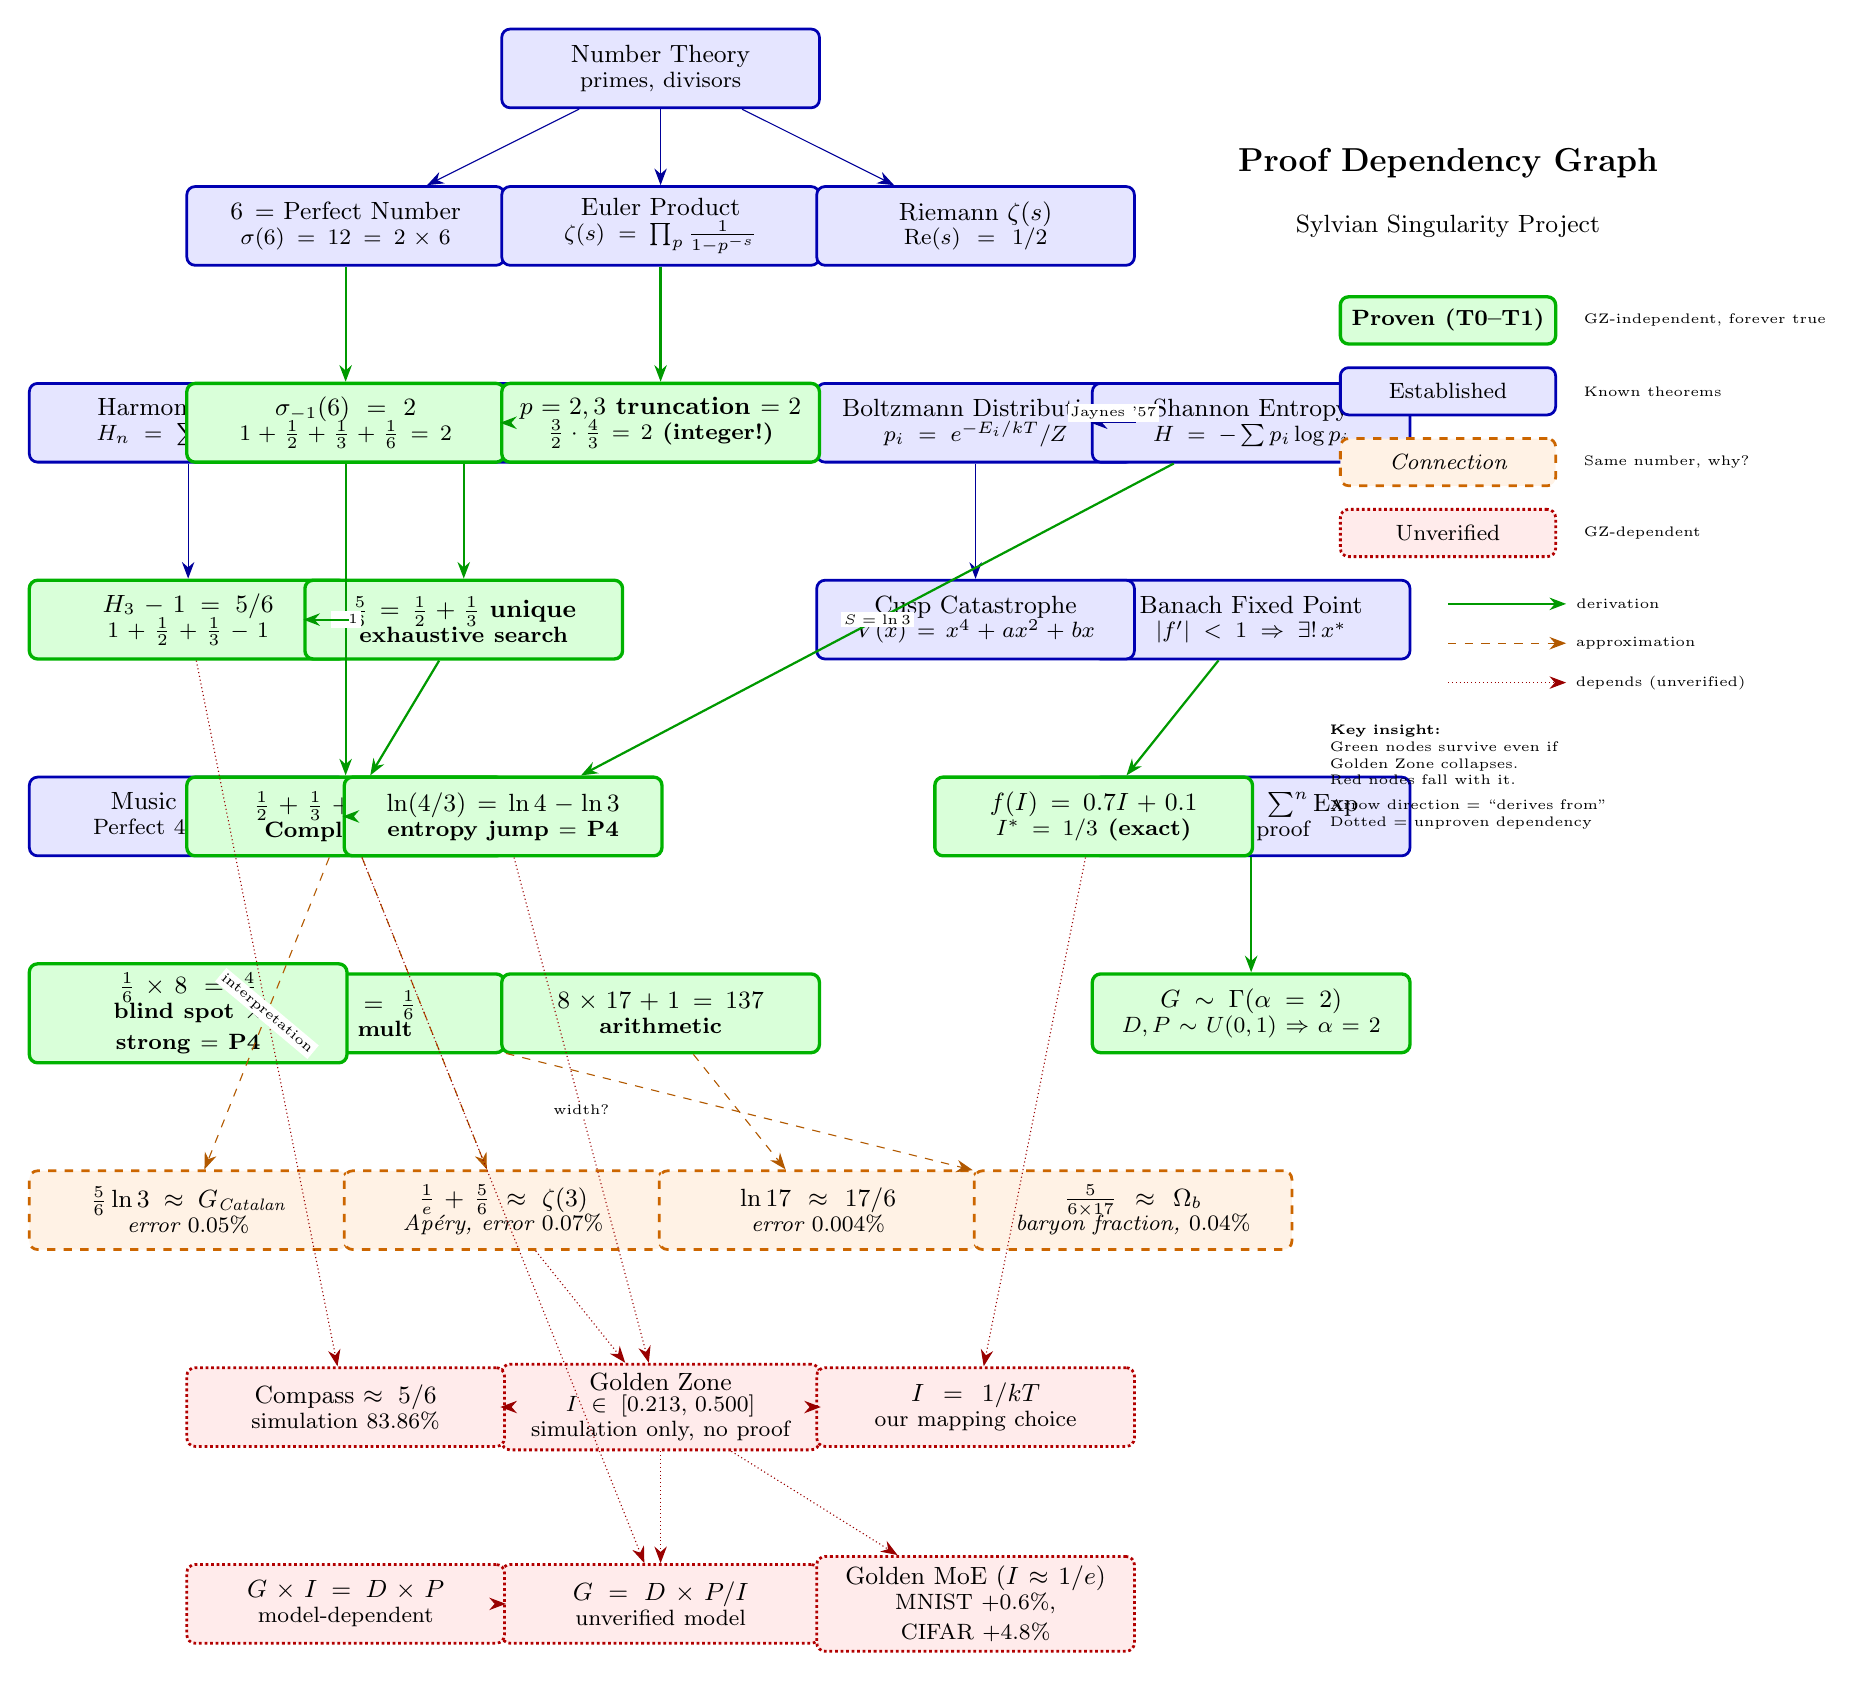
\begin{tikzpicture}[
    % Node styles by verification level
    proven/.style={
        rectangle, rounded corners=3pt, draw=green!70!black, fill=green!15,
        text width=3.8cm, align=center, font=\small\bfseries,
        minimum height=1cm, line width=1.2pt
    },
    established/.style={
        rectangle, rounded corners=3pt, draw=blue!70!black, fill=blue!10,
        text width=3.8cm, align=center, font=\small,
        minimum height=1cm, line width=1pt
    },
    connection/.style={
        rectangle, rounded corners=3pt, draw=orange!80!black, fill=orange!10,
        text width=3.8cm, align=center, font=\small\itshape,
        minimum height=1cm, line width=1pt, dashed
    },
    unverified/.style={
        rectangle, rounded corners=3pt, draw=red!70!black, fill=red!8,
        text width=3.8cm, align=center, font=\small,
        minimum height=1cm, line width=1pt, densely dotted
    },
    unfalsifiable/.style={
        rectangle, rounded corners=3pt, draw=purple!70!black, fill=purple!8,
        text width=3.8cm, align=center, font=\small,
        minimum height=1cm, line width=1pt, dotted
    },
    disproven/.style={
        rectangle, rounded corners=3pt, draw=black!60, fill=gray!15,
        text width=3.8cm, align=center, font=\small,
        minimum height=1cm, line width=1pt,
        text=black!50
    },
    % Arrow styles
    derives/.style={-{Stealth[length=6pt]}, thick, draw=green!60!black},
    uses/.style={-{Stealth[length=6pt]}, draw=blue!60!black},
    approx/.style={-{Stealth[length=6pt]}, dashed, draw=orange!70!black},
    depends/.style={-{Stealth[length=6pt]}, densely dotted, draw=red!60!black},
    % Label style
    elabel/.style={font=\tiny, fill=white, inner sep=1pt},
]

% ============================================================
% LAYER 1: Established Mathematics (Blue)
% ============================================================

\node[established] (numtheory) at (0, 0)
    {Number Theory\\[-2pt]\footnotesize primes, divisors};

\node[established] (perfect6) at (-4, -2)
    {$6 = $ Perfect Number\\[-2pt]\footnotesize $\sigma(6) = 12 = 2 \times 6$};

\node[established] (euler) at (0, -2)
    {Euler Product\\[-2pt]\footnotesize $\zeta(s) = \prod_p \frac{1}{1-p^{-s}}$};

\node[established] (riemann) at (4, -2)
    {Riemann $\zeta(s)$\\[-2pt]\footnotesize $\text{Re}(s) = 1/2$};

\node[established] (harmonic) at (-6, -4.5)
    {Harmonic Series\\[-2pt]\footnotesize $H_n = \sum_{k=1}^n 1/k$};

\node[established] (egyptian) at (-2.5, -4.5)
    {Egyptian Fractions\\[-2pt]\footnotesize unit fraction decomp.};

\node[established] (boltzmann) at (4, -4.5)
    {Boltzmann Distribution\\[-2pt]\footnotesize $p_i = e^{-E_i/kT}/Z$};

\node[established] (shannon) at (7.5, -4.5)
    {Shannon Entropy\\[-2pt]\footnotesize $H = -\sum p_i \log p_i$};

\node[established] (banach) at (7.5, -7)
    {Banach Fixed Point\\[-2pt]\footnotesize $|f'| < 1 \Rightarrow \exists!\, x^*$};

\node[established] (cusp) at (4, -7)
    {Cusp Catastrophe\\[-2pt]\footnotesize $V(x) = x^4 + ax^2 + bx$};

\node[established] (music) at (-6, -9.5)
    {Music Theory\\[-2pt]\footnotesize Perfect 4th $= 4/3$};

\node[established] (gamma) at (7.5, -9.5)
    {$\Gamma(n,\lambda) = \sum^n \text{Exp}$\\[-2pt]\footnotesize MGF proof};

% ============================================================
% LAYER 2: Proven (Green) - Pure math, GZ-independent
% ============================================================

\node[proven] (sigma6) at (-4, -4.5)
    {$\sigma_{-1}(6) = 2$\\[-2pt]\footnotesize $1+\frac{1}{2}+\frac{1}{3}+\frac{1}{6}=2$};

\node[proven] (euler23) at (0, -4.5)
    {$p=2,3$ truncation $=2$\\[-2pt]\footnotesize $\frac{3}{2}\cdot\frac{4}{3} = 2$ (integer!)};

\node[proven] (h3) at (-6, -7)
    {$H_3 - 1 = 5/6$\\[-2pt]\footnotesize $1+\frac{1}{2}+\frac{1}{3}-1$};

\node[proven] (egypt56) at (-2.5, -7)
    {$\frac{5}{6}=\frac{1}{2}+\frac{1}{3}$ unique\\[-2pt]\footnotesize exhaustive search};

\node[proven] (complete) at (-4, -9.5)
    {$\frac{1}{2}+\frac{1}{3}+\frac{1}{6}=1$\\[-2pt]\footnotesize Completeness};

\node[proven] (ln43) at (-2, -9.5)
    {$\ln(4/3) = \ln 4 - \ln 3$\\[-2pt]\footnotesize entropy jump $=$ P4};

\node[proven] (fixedpt) at (5.5, -9.5)
    {$f(I)=0.7I+0.1$\\[-2pt]\footnotesize $I^* = 1/3$ (exact)};

\node[proven] (constants) at (-4, -12)
    {$\frac{1}{2}\times\frac{1}{3}=\frac{1}{6}$\\[-2pt]\footnotesize sub $=$ mult};

\node[proven] (gammafit) at (7.5, -12)
    {$G \sim \Gamma(\alpha=2)$\\[-2pt]\footnotesize $D,P \sim U(0,1) \Rightarrow \alpha=2$};

\node[proven] (art137) at (0, -12)
    {$8\times 17+1=137$\\[-2pt]\footnotesize arithmetic};

\node[proven] (newgreen1) at (-6, -12)
    {$\frac{1}{6}\times 8 = \frac{4}{3}$\\[-2pt]\footnotesize blind spot $\times$ strong $=$ P4};

% ============================================================
% LAYER 3: Connections (Orange) - same number, why?
% ============================================================

\node[connection] (catalan) at (-6, -14.5)
    {$\frac{5}{6}\ln 3 \approx G_{\text{Catalan}}$\\[-2pt]\footnotesize error $0.05\%$};

\node[connection] (apery) at (-2, -14.5)
    {$\frac{1}{e}+\frac{5}{6} \approx \zeta(3)$\\[-2pt]\footnotesize Ap\'ery, error $0.07\%$};

\node[connection] (ln17) at (2, -14.5)
    {$\ln 17 \approx 17/6$\\[-2pt]\footnotesize error $0.004\%$};

\node[connection] (baryon) at (6, -14.5)
    {$\frac{5}{6\times 17} \approx \Omega_b$\\[-2pt]\footnotesize baryon fraction, $0.04\%$};

% ============================================================
% LAYER 4: Unverified (Red) - Golden Zone dependent
% ============================================================

\node[unverified] (goldenzone) at (0, -17)
    {Golden Zone\\[-2pt]\footnotesize $I \in [0.213,\, 0.500]$\\[-2pt]\footnotesize simulation only, no proof};

\node[unverified] (compass) at (-4, -17)
    {Compass $\approx 5/6$\\[-2pt]\footnotesize simulation $83.86\%$};

\node[unverified] (ikt) at (4, -17)
    {$I = 1/kT$\\[-2pt]\footnotesize our mapping choice};

\node[unverified] (gdpi) at (0, -19.5)
    {$G = D \times P / I$\\[-2pt]\footnotesize unverified model};

\node[unverified] (conserv) at (-4, -19.5)
    {$G \times I = D \times P$\\[-2pt]\footnotesize model-dependent};

\node[unverified] (goldenmoe) at (4, -19.5)
    {Golden MoE ($I \approx 1/e$)\\[-2pt]\footnotesize MNIST +0.6\%, CIFAR +4.8\%};

% ============================================================
% ARROWS: Derivation chains
% ============================================================

% Established → Established
\draw[uses] (numtheory) -- (perfect6);
\draw[uses] (numtheory) -- (euler);
\draw[uses] (numtheory) -- (riemann);
\draw[uses] (harmonic) -- (h3);
\draw[uses] (boltzmann) -- (cusp);

% Established → Proven
\draw[derives] (perfect6) -- (sigma6);
\draw[derives] (euler) -- (euler23);
\draw[derives] (egyptian) -- (egypt56);
\draw[derives] (banach) -- (fixedpt);
\draw[derives] (gamma) -- (gammafit);

% Proven → Proven
\draw[derives] (sigma6) -- node[elabel]{$-1$} (complete);
\draw[derives] (h3) -- (egypt56);
\draw[derives] (egypt56) -- (complete);
\draw[derives] (sigma6) -- (euler23);

% Proven → Connection (approximate)
\draw[approx] (complete) -- (catalan);
\draw[approx] (complete) -- (apery);
\draw[approx] (art137) -- (ln17);
\draw[approx] (constants) -- (baryon);

% Connection → Unverified
\draw[depends] (apery) -- (goldenzone);

% Proven → Unverified (interpretation gap)
\draw[depends] (h3) -- node[elabel, rotate=-40]{interpretation} (compass);
\draw[depends] (fixedpt) -- (ikt);
\draw[depends] (complete) -- (gdpi);
\draw[depends] (ln43) -- node[elabel]{width?} (goldenzone);

% Unverified internal
\draw[depends] (goldenzone) -- (gdpi);
\draw[depends] (gdpi) -- (conserv);
\draw[depends] (goldenzone) -- (goldenmoe);
\draw[depends] (ikt) -- (goldenzone);
\draw[depends] (compass) -- (goldenzone);

% Established → Proven (music-entropy connection)
\draw[derives] (music) -- (ln43);
\draw[derives] (shannon) -- node[elabel]{$S=\ln 3$} (ln43);

% Jaynes equivalence
\draw[uses] (boltzmann) -- (shannon) node[elabel, midway, above]{Jaynes '57};

% ============================================================
% LEGEND
% ============================================================

\begin{scope}[shift={(10, -2)}]
    \node[font=\large\bfseries] at (0, 0.8) {Proof Dependency Graph};
    \node[font=\small] at (0, 0) {Sylvian Singularity Project};

    \node[proven, text width=2.5cm, minimum height=0.6cm] at (0, -1.2) {\footnotesize Proven (T0--T1)};
    \node[font=\tiny, anchor=west] at (1.6, -1.2) {GZ-independent, forever true};

    \node[established, text width=2.5cm, minimum height=0.6cm] at (0, -2.1) {\footnotesize Established};
    \node[font=\tiny, anchor=west] at (1.6, -2.1) {Known theorems};

    \node[connection, text width=2.5cm, minimum height=0.6cm] at (0, -3.0) {\footnotesize Connection};
    \node[font=\tiny, anchor=west] at (1.6, -3.0) {Same number, why?};

    \node[unverified, text width=2.5cm, minimum height=0.6cm] at (0, -3.9) {\footnotesize Unverified};
    \node[font=\tiny, anchor=west] at (1.6, -3.9) {GZ-dependent};

    \draw[derives] (0, -4.8) -- ++(1.5, 0) node[font=\tiny, anchor=west]{derivation};
    \draw[approx] (0, -5.3) -- ++(1.5, 0) node[font=\tiny, anchor=west]{approximation};
    \draw[depends] (0, -5.8) -- ++(1.5, 0) node[font=\tiny, anchor=west]{depends (unverified)};

    \node[font=\tiny, text width=4cm, align=left] at (0.5, -7) {
        \textbf{Key insight:}\\
        Green nodes survive even if\\
        Golden Zone collapses.\\
        Red nodes fall with it.\\[3pt]
        Arrow direction = ``derives from''\\
        Dotted = unproven dependency
    };
\end{scope}

\end{tikzpicture}

\end{document}
